\label{sec:emissivity_sec}

A big problem in determining the viability of CSOs as UHECRs and neutrino sources is the problem of ion density and composition where the available data obtained through radio measurements or other wavelengths are attributed to electrons. Therefore, we need to investigate the ion density and composition of the emitting body. In this chapter we will outline an estimate of the ion density and composition based on jet propagation into the ambient medium,  make an estimate of the emissivity of UHECRs from the hotspots of CSOs, and lastly estimate the neutrino emissivity from the same sources.


\section{Ion density and composition}
The fraction of observed CSO $2.0,2.1$, and $2.2$ suggest that the deceleration phase between $2.0$ and $2.2$ happens quite rapidly. Given the lifetime of CSOs is on the order of $10^4$ years, the deceleration phase happens on a characteristic timescale of $10^3$ years. This is a very short timescale, and in \cite{sullivan2024smallscale} they propse a mechanism for the deceleration of the jet in both CSO $2.0$ and $2.1$ stages, which is mass loading. Mass loading is the process of the jet encountering various densities that supply an increase of mass to the jet, slowing it down sufficiently. In \cite{sullivan2024smallscale}, they find a relation that relates the deceleration time to lobe parameters based on a kinetic model, and is given as

\begin{equation}
    t \approx 1000\text{yr}\times \left(\frac{r_{b}}{10  \text{pc}}\right)^{-2} \left(\frac{M_p}{1 M_{\odot}}\right) \left(\frac{c_s }{250 \text{km/s}}\right)^{-1} \left(\frac{\rho_a}{10^{-24}\text{g cm}^{-3}}\right)^{-1}
\end{equation}

The example quoted in \cite{sullivan2024smallscale} takes a $1 M\odot$ lobe with a decleration timescale of $1000$ years and through conservation of momentum they find a required mass loading of $0.2 M_{\odot} \text{yr}^{-1}$. This loading rate can allow us to make simple estimates of the ion density that ends up in the lobes and that may experience acceleration. If the mass loading was caused by mass entrainment of the ambient medium, one can estimate the density that would suffice and in \cite{sullivan2024smallscale} setting $r=10$pc and $c_s = 250$km$/$s they find that an ambient density of $8\times 10^{-25} \text{g cm}^{-3}$ is needed to decelerate the jet. This density is similar in magnitude as the density found in elliptical galaxies cores according to \cite{Capelo_2010}. 

%The density calculated seems very low, but if one assumes an equal amount of protons and electron in the jet the intial mass density of the sphere would be $1.6\times 10^{-26}$ g cm$^{-3}$, meaning that the mass loading would 


Other sources of mass entrainment instead of the ambient density could be stellar mass loading, where the jet intercepts stellar objects. With this method we can estimate species composition as well which is less clear with ambient mass loading. For the following discussion, we will assume that the mass loading is caused by stellar objects.    
 By assuming that the mass loading is caused by stellar objects caught by the expanding jet, we can make some estimations. These objects will have a composition similar to the solar composition. The solar composition by mass is $74\%$ hydrogen, $24\%$ helium, and $2\%$ other elements. We can then estimate the number density of ions in the lobes assuming all mass loading ends up in the lobes via the following formula:

\begin{equation}
    n_{\text{ions}} = \frac{\dot{M} \times t_{l} }{\frac{4}{3} \pi R_{\text{lobe}}^3 (74\%m_p+24\%m_{\text{helium}}+2\%m_{\text{heavier ions}})}
\end{equation}

Setting $R = 10$ pc, $\dot{M} = 0.2 M\odot /$year, and $t_{l} = 1000$years we get the number density of ions to be $n_{\text{ions}} \approx 0.9  \text{cm}^{-3}$. This is a number density approximately equal in magnitude than that of the lowest density gas in the interestellar medium. We also receive the metallicity of the lobes, of $2\%$, which is the solar metallicity. The metallicity is not an unreasonable number but is purley based on the assumption that the mass loading is caused by stellar objects. One important assumption is that the stellar mass loading is in the form of gas that distributes itself over the lobe. A more realistic model of mass entrainment would need to investigate the affect the jet can have one the star. Our result here is with the intent of estimating a type of composition, and the number density of ions in the lobe. 

 

%\cite{sullivan2024smallscale} find that the number of stars needed for the...


\section{UHECRs Emissivity}
\label{sec:emissivity_mass_load}
In the previous sections we have estimate the possible maximum energy achieved by a proton, the number density of CSOs, and lastly the number density and composition of ions due to mass loading. With this information and given a few assumptions on the energy spectra of the protons, we can estimate the emissivity of UHECRs from these sources.

The energy spectrum of protons undergoing first-order acceleration is usually a power law with spectral index $\alpha = 2$, but in order to incorporate energy losses one commenly use a broken power law to describe the spectrum, and a harder spectral index. The broken power law spectrum of the number of protons per unit energy is given by:

\begin{equation}
    \label{eq:proton_spectrum}
    N(\gamma) = \begin{cases}
    N_0 \gamma^{-\alpha} & \gamma < \gamma_{\text{break}} \\
    N_0 \gamma_{\text{break}}\gamma^{-\alpha-1} & \gamma > \gamma_{\text{break}}
    \end{cases}
\end{equation}

By arguing that the number of ions in the lobe is equal to the total mass loaded into the lobe, $V_{\text{lobe}} n_{\text{Ion}} = \int_{\gamma_{\text{min}}}^{\gamma_{\text{max}}} N(\gamma) d\gamma$, we can normalize the spectrum.  We can separate the number of ions into those of different species by multiplying with the percentage of the mass that is of that species. With this, we can estimate the internal energy of any desired species in the lobe. $\gamma_{\text{max}}$ is estimated based on the maximum energy of the particular species. The total internal energy of any species in the lobe can then be calculated as,

\begin{equation}
    U_{\text{I}} = m_i c^2 \int_{\gamma_{\text{min}}}^{\gamma_{\text{max}}} \gamma N(\gamma)d\gamma
\end{equation}

By assuming that all internal energy is converted to UHECRs and radiated away at a constant rate, we can estimate the luminosity of cosmic rays as $L_{\text{species}} = U_{\text{species}}/t_{\text{life}}$. In order to calculate the specific luminosity of UHECRs we separate the internal energy stored in all ions to those of the most energetic by calculating the separate internal energy for UHECRs. That is to say, only ions with energy larger than $\gamma > 10^{10}$. Using our estimate of the density of CSO $2.0$s at $10^{-5} \text{Mpc}^{-3}$, $\gamma_{\text{max}} = \frac{3 \times 10^{19} \times Z}{m_p c^2}$ and $\gamma_{\text{min}} = 1$,$\alpha =2.47$, $\gamma_{\text{break}}= 10^6$ , we can estimate the emissivity of UHECRs per species as $Q_{\text{UHECR}} = L_{\text{species}} n_{\text{CSO}}$. The value of $\alpha$ and $\gamma_{\text{break}}$ are derived by estimating that the energy loss of protons increases the original spectral index by $0.47$ and the break energy is caused by less efficient acceleration at higher energies.

The results of the calculations can be seen in table \ref{tab:emissivity_mass_load}.

\begin{table}[H]
    \centering
    \begin{tabular}{|c|c|c|c|}
    \hline
    \textbf{Variable} & \textbf{Protons} & \textbf{Helium} & \textbf{Heavier Ions} \\
    \hline
    \textbf{$u$ (erg cm$^{-3}$)} & \(1.9 \times 10^{-12}\) & \(2.5 \times 10^{-12}\) & \(1.4 \times 10^{-12}\) \\
    \hline
    \textbf{L (erg s$^{-1}$)} & \(2.3 \times 10^{47}\) & \(3.0 \times 10^{47}\) & \(1.7 \times 10^{47}\) \\
    \hline
    \textbf{$\epsilon$ (erg Mpc$^{-3}$ yr$^{-1}$)} & \(8.8 \times 10^{49}\) & \(1.1 \times 10^{50}\) & \(6.4 \times 10^{49}\) \\
    \hline
    \textbf{$u_{\text{UHECRs}}$ (erg cm$^{-3}$)} & \(9.6 \times 10^{-20}\) & \(1.2\times 10^{-19}\) & \(7.0 \times 10^{-20}\) \\
    \hline
    \textbf{$L_{\text{UHECRs}}$ (erg s$^{-1}$)} & \(1.2 \times 10^{40}\) & \(1.5 \times 10^{40}\) & \(8.6 \times 10^{39}\) \\
    \hline
    \textbf{$\epsilon_{\text{UHECRs}}$  (erg Mpc$^{-3}$ yr$^{-1}$)} & \(4.5 \times 10^{42}\) & \(5.8 \times 10^{42}\) & \(3.3 \times 10^{42}\) \\
    \hline
    \end{tabular}
    \caption{Mass Loading and Extra-Galactic Results for Different Species}
    \label{tab:emissivity_mass_load}
\end{table}
 
The values of the calculation give reasonable values for the emissivity of UHECRs, but not reasonable values for the luminosity of all protons. The luminosity of the protons is a factor $100$ higher than the most powerful jet in figure \ref{fig:jet_power} which makes this unphysical. The average ion density is very low,  but this is a consequence of very efficient mass shedding via CR acceleration. One preformed the same test by equating the ion energy density to the magnetic field density, and the results can be seen in the Appendix. 
%And this is still under the assumption of a very low estimate for the ion density. In addition, we check for a different scenario in which we equates the ion energy density to the magnetic field density. Again the magnetic field density is given as $u_B = \frac{B^2 }{ 8 \pi} = 3.98 \times 10^{-6}$ for a magnetic field of $B = 10^{-2}$ G. The results of this assumption can be seen in table \ref{tab:emissivity_mass_load_B}. 




%Here we has a overshot the emissivity of UHECRs when comparing it to the measured emissivity discussed in section \ref{sec:emmisivity}, with the emissivity of UHECRs being of the order of $5\times 10^{46}$ erg Mpc$^{-3}$ yr$^{-1}$. These values are incedibly high and are unreasonable to this extent that one does not see this type of local emissivity. With this argument it becomes clearer that equating the ion density to the magnetic field density might not be necessary. The result in table \ref{tab:emissivity_mass_load_B} is contingent on the emission region since a bigger emission region will allow for higher number of ions, but the table in \ref{tab:emissivity_mass_load} is only contingent on the mass loaded by stellar mass loading. The emissivity of UHECRs from the stellar mass loading argument would be approximately $2\%$ of the total emissivity. This is a reasonable number, that could be higher if paramters such as ion density, CSO number density, or mangetic field strength are higher.

Both these results overshoot their total comsic ray luminosity since the CR luminosity is higher than even the highest jet power. This makes the result unreasonable, and one should almost certainly tweek our paramters. It is clear that if all entrained mass, stellar or from the ambient density ends up in the lobes, and is accelerated the luminosity will be too high. We argue that not all mass ends up being accelerated. In order for the UHECRs luminosity to be of significant values and keeping the luminosity of CR at a reasonable value one should consider two things. Firstly that not all mass is accelerated and escapes. The consequence of this is that most entrained mass will be cold protons that follow the jet, and do not escpae the system in our given time frame. Secondly one would like to consider a softer spectrum of protons, which will increase the relative emission of UHECRs. If this is reasonable is not yet clear but allows for comparison. We run the model on this biased choice of parameters. We  assume that only $0.01\%$ of the mass loaded into the lobe is accelerated, and only a single power law spectrum for our protons with $\alpha = 2.47$. The result of this configuration can be seen in table \ref{tab:emissivity_mass_load_1}.
\begin{table}[H]
    \centering
    \begin{tabular}{|c|c|c|c|}
    \hline
    \textbf{Variable} & \textbf{Protons} & \textbf{Helium} & \textbf{Heavier Ions} \\
    \hline
    \textbf{$u$ (erg cm$^{-3}$)} & \(4.8 \times 10^{-4}\) & \(6.2 \times 10^{-4}\) & \(3.5 \times 10^{-4}\) \\
    \hline
    \textbf{L (erg s$^{-1}$)} & \(2.3 \times 10^{44}\) & \(3.0 \times 10^{44}\) & \(1.7 \times 10^{44}\) \\
    \hline
    \textbf{$\epsilon$ (erg Mpc$^{-3}$ yr$^{-1}$)} & \(8.9 \times 10^{46}\) & \(1.1 \times 10^{47}\) & \(6.5 \times 10^{46}\) \\
    \hline
    \textbf{$u_{\text{UHECRs}}$ (erg cm$^{-3}$)} & \(2.7 \times 10^{-19}\) & \(4.2 \times 10^{-19}\) & \(2.3 \times 10^{-19}\) \\
    \hline
    \textbf{$L_{\text{UHECRs}}$ (erg s$^{-1}$)} & \(3.3 \times 10^{40}\) & \(5.1 \times 10^{40}\) & \(2.9 \times 10^{40}\) \\
    \hline
    \textbf{$\epsilon_{\text{UHECRs}}$  (erg Mpc$^{-3}$ yr$^{-1}$)} & \(1.3 \times 10^{43}\) & \(1.9 \times 10^{43}\) & \(1.1 \times 10^{43}\) \\
    \hline
    \end{tabular}
    \caption{Emissivity of CR and UHECRs for different species with a single powerlaw spectrum and a low percent of mass loaded into the lobe expericening acceleration.}
    \label{tab:emissivity_mass_load_1}
\end{table}


Our results have succeeded in lowering the luminosity of CR with an added cost of significantly increasing the energy density of ions in the lobes, due to the cold protons introduced. The energy density of our magnetic field in this scenario is of the order $10^{-6}$ meaning that the remaining energy density of cold protons is quite high. The comparisson between the two cases hints at an equilibrium where the ion density of ions does not get too high due to the radiative efficiency of the lobe of dispelling them. This is hypothetical, but with the fact that the lobe would most likely entrain mass, a good question is what happens to those ions.
The observation we derive from this is that the lobes of CSOs have a viable source of ions which can be accelerated to CR. The additonal observation is that with this model with parameters taken from \cite{sullivan2024smallscale} the non acceleration of entrained mass will likely lead to a high energy density of ions in the lobes. 

One assumed a stellar composition of the mass loaded into the lobe in order to study the distribution of emissivity across species. The results show that the species distributed emissivities are of equal order magnetiude with helium ions carrying the most energy out. Therefore, if the compositon of UHECRs in the hotspots include helium ions, and heavier ions it is reasonable to assume that they will carry a substantial amount of the energy out of the system. 


 

%\subsection{Motivation for luminosity of UHECRs}
%In order to look for luminosity of UHECRs from the lobes, we argue that the energy budget of the jet can reveal some interesting dynamics.  We argue that in the system of the lobe expansion into the ambient medium the energy calculation should be a zero if one includes all sources of loss. The equation for the resulting power budget in the jet can be written as 





\section{Neutrino Emissivity}
Lastly, we might like to look for neutrinos from the same sources as the UHECRs. We aim here to calculate the expected fraction of neutrinos produced via the photopion effect in the hotspots of the CSO from the escaping protons. From our estimate of the photopion timescale in the previous sections, we can estimate the resulting flux of neutrinos as a relation to the escaping protons. The methodology is taken from \cite{Oikonomou_2019}.
Given the number of protons escaping the system, one can estimate the number of neutrinos produced as

\begin{equation}
\epsilon_{\nu}^2 \frac{dN_{\nu}}{d\epsilon_{\nu}} = \frac{1}{4} f_{p\gamma}f_{\pi, \text{cool}} f_{\mu,\text{cool}}\epsilon_p^2 \frac{dN_{p}}{d\epsilon_{p}}
\end{equation}

where $f_{p\gamma}$ is the fraction of lost protons that undergo the photopion interaction defined as, $f_{p\gamma} = t_{p\gamma}/t_{\text{cool}}$, $f_{\pi, \text{cool}}$ and $f_{\mu, \text{cool}}$ are suppression factors that take into account energy loss from pions and muons respectively defined as $f_{\pi, \text{cool}} = 1-\exp{(-t_{\pi,\text{cool}}/t_{\pi, \text{dec}})}$. Where $t_{\pi,\text{cool}} = t_{\pi, \text{syn}} + t_{\text{dyn}}$, $t_{\pi, \text{dec}} = \gamma_{\pi}\tau_{\pi}$ with $\tau_{\pi} = 2.6\times 10^{-8}$ and $\tau_{\mu} = 2.2\times 10^{-6}$.

One is not intending on finding the specific neutrino flux since the prefactor will illuminate the desired trend of the system. The energy-dependent prefactor can be seen in figure \ref{fig:neutrino_flux_prefactor}.

\begin{figure}
    \centering
    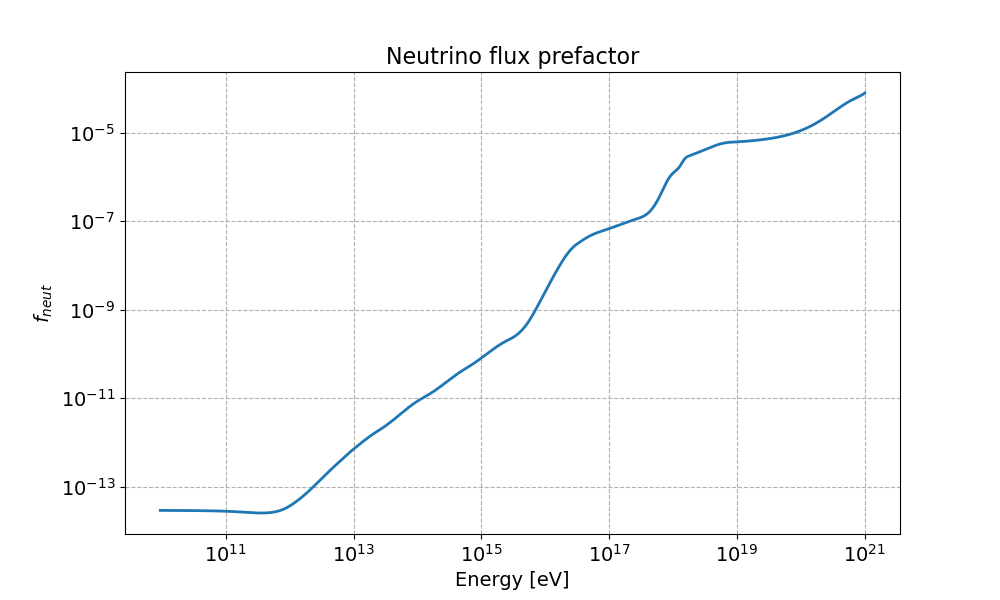
\includegraphics[width=0.8\textwidth]{C:/Users/henri/OneDrive/Documents/NTNU/Semester 10/Masteroppgave/Plots/Neutrino_flux_prefactor.png}
    \caption{Energy-dependent prefactor for the neutrino flux as a function proton losses. The prefactor is calculated for CSO hotspots, and the photopion effect from figure \ref{fig:timescales}.}
\label{fig:neutrino_flux_prefactor}
\end{figure}

Here one sees that the maximum ratio of proton flux to neutrino flux is around $10^{-5}$, a significantly low number. Due to the fact that the emissivity of UHECRs and neutrinos are of the same order of magnitude, one can conclude that the neutrino flux from the CSO hotspots is not significant. This is not surprising since the photopion losses are not dominating the acceleration. But there is still a case to be made for the CSO core, which is not covered here.

